\documentclass[10pt]{article}\usepackage[]{graphicx}\usepackage[]{xcolor}
% maxwidth is the original width if it is less than linewidth
% otherwise use linewidth (to make sure the graphics do not exceed the margin)
\makeatletter
\def\maxwidth{ %
  \ifdim\Gin@nat@width>\linewidth
    \linewidth
  \else
    \Gin@nat@width
  \fi
}
\makeatother

\definecolor{fgcolor}{rgb}{0.345, 0.345, 0.345}
\newcommand{\hlnum}[1]{\textcolor[rgb]{0.686,0.059,0.569}{#1}}%
\newcommand{\hlsng}[1]{\textcolor[rgb]{0.192,0.494,0.8}{#1}}%
\newcommand{\hlcom}[1]{\textcolor[rgb]{0.678,0.584,0.686}{\textit{#1}}}%
\newcommand{\hlopt}[1]{\textcolor[rgb]{0,0,0}{#1}}%
\newcommand{\hldef}[1]{\textcolor[rgb]{0.345,0.345,0.345}{#1}}%
\newcommand{\hlkwa}[1]{\textcolor[rgb]{0.161,0.373,0.58}{\textbf{#1}}}%
\newcommand{\hlkwb}[1]{\textcolor[rgb]{0.69,0.353,0.396}{#1}}%
\newcommand{\hlkwc}[1]{\textcolor[rgb]{0.333,0.667,0.333}{#1}}%
\newcommand{\hlkwd}[1]{\textcolor[rgb]{0.737,0.353,0.396}{\textbf{#1}}}%
\let\hlipl\hlkwb

\usepackage{framed}
\makeatletter
\newenvironment{kframe}{%
 \def\at@end@of@kframe{}%
 \ifinner\ifhmode%
  \def\at@end@of@kframe{\end{minipage}}%
  \begin{minipage}{\columnwidth}%
 \fi\fi%
 \def\FrameCommand##1{\hskip\@totalleftmargin \hskip-\fboxsep
 \colorbox{shadecolor}{##1}\hskip-\fboxsep
     % There is no \\@totalrightmargin, so:
     \hskip-\linewidth \hskip-\@totalleftmargin \hskip\columnwidth}%
 \MakeFramed {\advance\hsize-\width
   \@totalleftmargin\z@ \linewidth\hsize
   \@setminipage}}%
 {\par\unskip\endMakeFramed%
 \at@end@of@kframe}
\makeatother

\definecolor{shadecolor}{rgb}{.97, .97, .97}
\definecolor{messagecolor}{rgb}{0, 0, 0}
\definecolor{warningcolor}{rgb}{1, 0, 1}
\definecolor{errorcolor}{rgb}{1, 0, 0}
\newenvironment{knitrout}{}{} % an empty environment to be redefined in TeX

\usepackage{alltt}
\usepackage[left=1in,right=1in,top=1in,bottom=1in]{geometry}
\usepackage{amsmath}
\usepackage{hyperref}
%\SweaveOpts[concordance=TRUE]
\IfFileExists{upquote.sty}{\usepackage{upquote}}{}
\begin{document}

\begin{titlepage}
    \centering
    
    { \Huge \textbf{Final Project Report Draft 1} \par} 
    \vspace{5mm}
    { \huge \textbf{Motor vehicle colisions in NYC} \par} 
    \vspace{3mm}
    { \Large Group 1 (STAT 605 - S1)\par}  
    
    \vspace{5mm}
    \begin{center}
    \line(1,0){425}
    \end{center}
    
    \vspace{5mm}

    \vspace{15mm}
    { \large Authors: \par }
      \vspace{3mm}
    { \Large \textbf{Astha Singh} - \texttt{as677@rice.edu} \par}
    { \Large \textbf{Franco Bosetti} - \texttt{fb57@rice.edu}\par}
    { \Large \textbf{Louis Clarke} - \texttt{lc160@rice.edu}\par}
    { \Large \textbf{Lindsey Russ} - \texttt{ltr1@rice.edu}\par}    
    
    
    \vspace{5mm}
    \date{\today}
    
    \vspace{5mm}

\end{titlepage}

\newpage


\tableofcontents

\newpage

\section{Introduction}

Motor vehicle collisions are a major concern in major populated urban areas like New York City (NYC), where millions of people use diverse transportation systems every day. Understanding these incidents through data analysis can help us identify patterns and make safety improvements. On the other hand, social media platforms such as Twitter have become spaces where people share their real-time information about traffic incidents and congestion. This project will analyze motor vehicle collision data in NYC and explore the relationship between actual incidents and social media traffic discussions. 

\section{Dataset Description}
Primary Dataset: NYC Motor Vehicle Collisions 

(\url{https://data.cityofnewyork.us/Public-Safety/Motor-Vehicle-Collisions-Crashes/h9gi-nx95/about_data})

Our primary dataset contains police-reported motor vehicle collision records from New York City, maintained by the NYPD through their TrafficStat initiative. The dataset includes 2.21 million collision records with 29 variables.


Source: NYC OpenData (2025)


Key variables include:
\begin{itemize}
  \item Location \& Time: Borough, coordinates (latitude \& longitude), street names, zip codes, crash date/time
  \item Casualties: Injuries and fatalities by category (pedestrians, cyclists, motorists)
  \item Contributing Factors: Up to five causal factors per collision
  \item Vehicle Types: Vehicle type classifications (ATV, bicycle, car/SUV, e-bike, e-scooter, truck/bus, motorcycle, other) for each vehicle involved
\end{itemize}


Preprocessing: We prepared the dataset for analysis by converting crash dates to a standard date format, organizing borough names as categorical variables, and creating additional time-based variables to explore patterns across years and months. 

Secondary Dataset: Twitter Traffic Classifications (\url{https://data.mendeley.com/datasets/c3xvj5snvv/1})

Our secondary dataset contains classified tweets collected from Twitter's API, with each tweet categorized by its traffic-related content.


Source: Research dataset by Sina Dabiri (2018)


Variables include:
\begin{itemize}
  \item Tweet ID
  \item Classification label: 
  \item Non-Traffic (Class 0): General tweets unrelated to traffic
  \item Traffic Incident (Class 1): Reports of crashes, breakdowns, road closures
  \item Traffic Conditions (Class 2): Congestion reports, traffic advisories, flow conditions
  \item Tweet text content
\end{itemize}

Preprocessing: We haven't processed the Twitter data yet, but plan to rename variables and clean the text data to prepare it for our analysis and comparison with the collision records.

\newpage


\section{Visualizations}

Prepare the data for processing:

\begin{knitrout}
\definecolor{shadecolor}{rgb}{0.969, 0.969, 0.969}\color{fgcolor}\begin{kframe}
\begin{alltt}
\hldef{nyc} \hlkwb{<-} \hlkwd{read.csv}\hldef{(}\hlkwc{file} \hldef{=} \hlsng{"data/Motor_Vehicle_Collisions_-_Crashes.csv"}\hldef{)}
\hldef{nyc}\hlopt{$}\hldef{CRASH.DATE} \hlkwb{<-} \hlkwd{as.Date}\hldef{(nyc}\hlopt{$}\hldef{CRASH.DATE,} \hlkwc{format} \hldef{=} \hlsng{"%m/%d/%Y"}\hldef{)}
\hldef{nyc}\hlopt{$}\hldef{BOROUGH} \hlkwb{<-} \hlkwd{factor}\hldef{(nyc}\hlopt{$}\hldef{BOROUGH)}
\hldef{nyc}\hlopt{$}\hldef{YEAR_MONTH} \hlkwb{<-} \hlkwd{format}\hldef{(nyc}\hlopt{$}\hldef{CRASH.DATE,} \hlsng{"%Y-%m"}\hldef{)}
\hldef{nyc}\hlopt{$}\hldef{YEAR} \hlkwb{<-} \hlkwd{format}\hldef{(nyc}\hlopt{$}\hldef{CRASH.DATE,} \hlsng{"%Y"}\hldef{)}
\end{alltt}
\end{kframe}
\end{knitrout}

\subsection{Vehicle Collisions over Time}
By grouping the collisions into each month in which they occured, we can plot a line graph showing the number of collisions over the past 13 years.
\begin{knitrout}
\definecolor{shadecolor}{rgb}{0.969, 0.969, 0.969}\color{fgcolor}\begin{kframe}
\begin{alltt}
\hldef{monthly_counts} \hlkwb{<-} \hlkwd{table}\hldef{(nyc}\hlopt{$}\hldef{YEAR_MONTH)}
\hldef{months} \hlkwb{<-} \hlkwd{names}\hldef{(monthly_counts)}
\hldef{colspermonth} \hlkwb{<-} \hlkwd{as.numeric}\hldef{(monthly_counts)}
\hldef{plot_months} \hlkwb{<-} \hlkwd{as.Date}\hldef{(}\hlkwd{paste0}\hldef{(months,} \hlsng{"-01"}\hldef{))}
\hlkwd{plot}\hldef{(plot_months, colspermonth,}
     \hlkwc{main}\hldef{=}\hlsng{"Number of Monthly Vehicle Collisions in New York City"}\hldef{,}
     \hlkwc{type}\hldef{=}\hlsng{"o"}\hldef{,}
     \hlkwc{pch}\hldef{=}\hlnum{20}\hldef{,}
     \hlkwc{xlab}\hldef{=}\hlsng{"Month"}\hldef{,}
     \hlkwc{ylab}\hldef{=}\hlsng{"Number of Collisions"}\hldef{,}
     \hlkwc{xaxt}\hldef{=}\hlsng{"n"}\hldef{,}
     \hlkwc{yaxt}\hldef{=}\hlsng{"n"}\hldef{,}
     \hlkwc{xaxs}\hldef{=}\hlsng{"i"}\hldef{,}
     \hlkwc{yaxs}\hldef{=}\hlsng{"i"}\hldef{,}
     \hlkwc{ylim}\hldef{=}\hlkwd{c}\hldef{(}\hlnum{0}\hldef{,}\hlkwd{max}\hldef{(colspermonth)}\hlopt{+}\hlnum{1000}\hldef{))}


\hldef{xticks} \hlkwb{<-} \hlkwd{seq}\hldef{(}\hlkwd{min}\hldef{(plot_months),} \hlkwd{max}\hldef{(plot_months)}\hlopt{+}\hlnum{365}\hldef{,} \hlkwc{by} \hldef{=} \hlsng{"6 months"}\hldef{)}
\hlkwd{axis.Date}\hldef{(}\hlnum{1}\hldef{,} \hlkwc{at} \hldef{= xticks,}
          \hlkwc{format} \hldef{=} \hlsng{"%b\textbackslash{}n%Y"}\hldef{,} \hlkwc{cex.axis} \hldef{=} \hlnum{0.6}\hldef{)}
\hlkwd{axis}\hldef{(}\hlnum{2}\hldef{,} \hlkwc{at} \hldef{=} \hlkwd{seq}\hldef{(}\hlnum{0}\hldef{,} \hlkwd{max}\hldef{(colspermonth)}\hlopt{+}\hlnum{1000}\hldef{,} \hlkwc{by} \hldef{=} \hlnum{1000}\hldef{),} \hlkwc{cex.axis} \hldef{=} \hlnum{0.7}\hldef{,} \hlkwc{las}\hldef{=}\hlnum{1}\hldef{)}
\hlkwd{abline}\hldef{(}\hlkwc{v} \hldef{= xticks,} \hlkwc{col} \hldef{=} \hlsng{"gray"}\hldef{,} \hlkwc{lty} \hldef{=} \hlsng{"dotted"}\hldef{)}
\end{alltt}
\end{kframe}
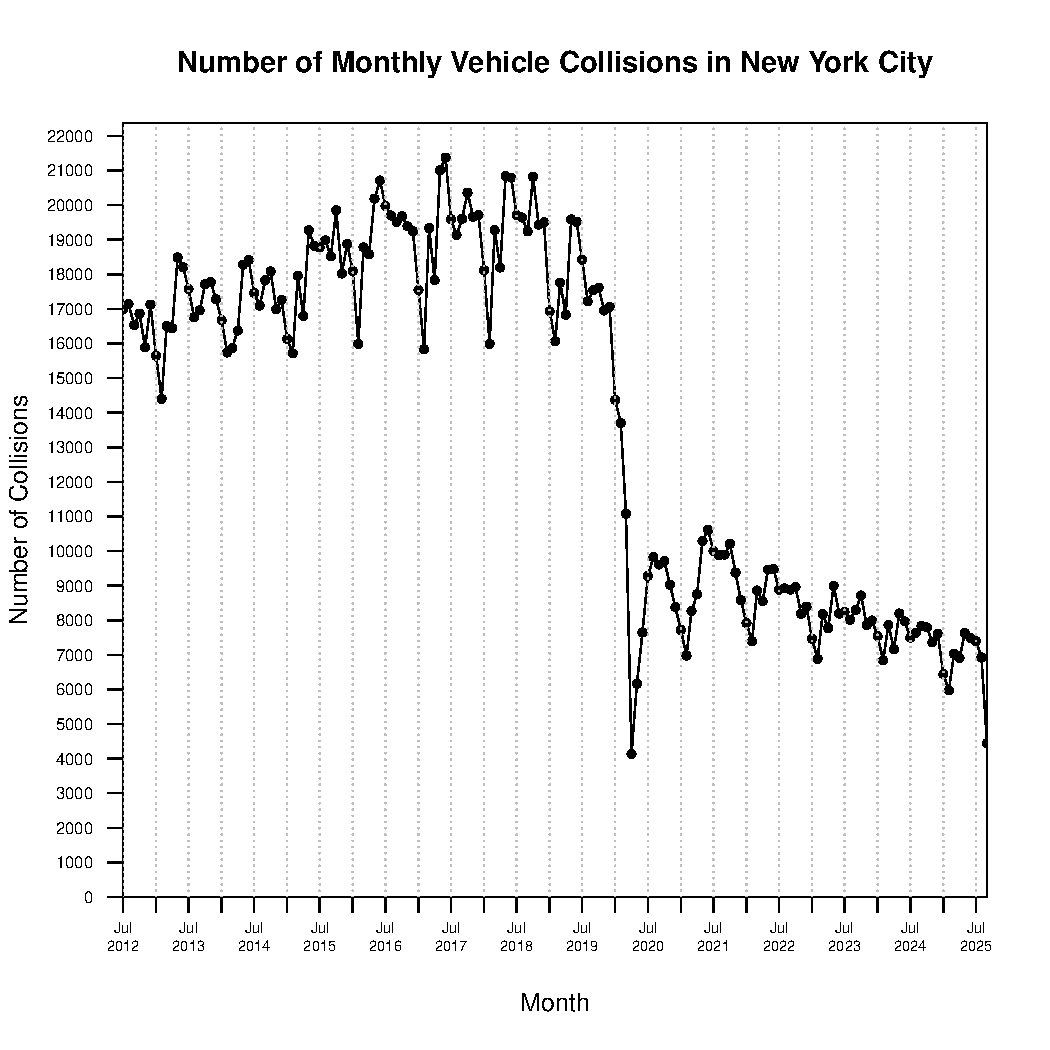
\includegraphics[width=\maxwidth]{figure/unnamed-chunk-2-1} 
\end{knitrout}
A notable trend is the sudden drop in collisions at the beginning of 2020. This is clearly due to the Covid-19 pandemic, which limited the time people spent outside their homes. What is more notable is how the number of collisions seems to even out to a much lower level than pre-pandemic. More research is needed into why we see this pattern.
\\ \\
Next, we explore the number of collisions over time within each borough. Note that a large quantity of entries from the dataset do not have a location attached, so those results are not considered for this analysis.
\begin{knitrout}
\definecolor{shadecolor}{rgb}{0.969, 0.969, 0.969}\color{fgcolor}\begin{kframe}
\begin{alltt}
\hldef{borough} \hlkwb{<-} \hlkwd{levels}\hldef{(nyc}\hlopt{$}\hldef{BOROUGH)}
\hldef{borough} \hlkwb{<-} \hldef{borough[borough} \hlopt{!=} \hlsng{""}\hldef{]}
\hldef{colors} \hlkwb{=} \hlkwd{c}\hldef{(}\hlsng{"red"}\hldef{,} \hlsng{"blue"}\hldef{,} \hlsng{"darkgreen"}\hldef{,} \hlsng{"purple"}\hldef{,} \hlsng{"orange"}\hldef{)}
\hldef{plot_months} \hlkwb{<-} \hlkwd{list}\hldef{()}
\hldef{colspermonth} \hlkwb{<-} \hlkwd{list}\hldef{()}
\hlkwa{for} \hldef{(b} \hlkwa{in} \hldef{borough)\{}
  \hldef{monthly_counts} \hlkwb{<-} \hlkwd{table}\hldef{(nyc}\hlopt{$}\hldef{YEAR_MONTH[nyc}\hlopt{$}\hldef{BOROUGH}\hlopt{==}\hldef{b])}
  \hldef{months} \hlkwb{<-} \hlkwd{names}\hldef{(monthly_counts)}
  \hldef{colspermonth[[b]]} \hlkwb{<-} \hlkwd{as.numeric}\hldef{(monthly_counts)}
  \hldef{plot_months[[b]]} \hlkwb{<-} \hlkwd{as.Date}\hldef{(}\hlkwd{paste0}\hldef{(months,} \hlsng{"-01"}\hldef{))}
\hldef{\}}

\hldef{max_col} \hlkwb{<-} \hlkwd{max}\hldef{(}\hlkwd{sapply}\hldef{(colspermonth, max))}
\hldef{min_dat} \hlkwb{<-} \hlkwd{as.Date}\hldef{(}\hlkwd{min}\hldef{(}\hlkwd{sapply}\hldef{(plot_months,min)))}
\hldef{max_dat} \hlkwb{<-} \hlkwd{as.Date}\hldef{(}\hlkwd{max}\hldef{(}\hlkwd{sapply}\hldef{(plot_months,max)))}

\hlkwd{plot}\hldef{(plot_months[[}\hlnum{1}\hldef{]], colspermonth[[}\hlnum{1}\hldef{]],}
     \hlkwc{main}\hldef{=}\hlsng{"Number of Monthly Vehicle Collisions in New York City"}\hldef{,}
     \hlkwc{type}\hldef{=}\hlsng{"l"}\hldef{,}
     \hlkwc{pch}\hldef{=}\hlnum{20}\hldef{,}
     \hlkwc{col}\hldef{= colors[}\hlnum{1}\hldef{],}
     \hlkwc{xlab}\hldef{=}\hlsng{"Month"}\hldef{,}
     \hlkwc{ylab}\hldef{=}\hlsng{"Number of Collisions"}\hldef{,}
     \hlkwc{xaxt}\hldef{=}\hlsng{"n"}\hldef{,}
     \hlkwc{yaxt}\hldef{=}\hlsng{"n"}\hldef{,}
     \hlkwc{xaxs}\hldef{=}\hlsng{"i"}\hldef{,}
     \hlkwc{yaxs}\hldef{=}\hlsng{"i"}\hldef{,}
     \hlkwc{ylim}\hldef{=}\hlkwd{c}\hldef{(}\hlnum{0}\hldef{,max_col}\hlopt{+}\hlnum{500}\hldef{))}

\hlkwa{for} \hldef{(i} \hlkwa{in} \hlnum{2}\hlopt{:}\hldef{(}\hlkwd{length}\hldef{(borough)))\{}
  \hlkwd{lines}\hldef{(plot_months[[i]], colspermonth[[i]],} \hlkwc{type}\hldef{=}\hlsng{"l"}\hldef{,} \hlkwc{pch}\hldef{=}\hlnum{20}\hldef{,} \hlkwc{col}\hldef{=colors[i])}
\hldef{\}}

\hlkwd{legend}\hldef{(}\hlsng{"topright"}\hldef{,}
       \hlkwc{legend} \hldef{= borough,}
       \hlkwc{col} \hldef{= colors,}
       \hlkwc{lty} \hldef{=} \hlnum{1}\hldef{)}


\hldef{xticks} \hlkwb{<-} \hlkwd{seq}\hldef{(min_dat, max_dat}\hlopt{+}\hlnum{365}\hldef{,} \hlkwc{by} \hldef{=} \hlsng{"6 months"}\hldef{)}
\hlkwd{axis.Date}\hldef{(}\hlnum{1}\hldef{,} \hlkwc{at} \hldef{= xticks,}
          \hlkwc{format} \hldef{=} \hlsng{"%b\textbackslash{}n%Y"}\hldef{,} \hlkwc{cex.axis} \hldef{=} \hlnum{0.6}\hldef{)}
\hlkwd{axis}\hldef{(}\hlnum{2}\hldef{,} \hlkwc{at} \hldef{=} \hlkwd{seq}\hldef{(}\hlnum{0}\hldef{, max_col}\hlopt{+}\hlnum{1000}\hldef{,} \hlkwc{by} \hldef{=} \hlnum{1000}\hldef{),} \hlkwc{cex.axis} \hldef{=} \hlnum{0.7}\hldef{,} \hlkwc{las}\hldef{=}\hlnum{1}\hldef{)}
\hlkwd{abline}\hldef{(}\hlkwc{v} \hldef{= xticks,} \hlkwc{col} \hldef{=} \hlsng{"gray"}\hldef{,} \hlkwc{lty} \hldef{=} \hlsng{"dotted"}\hldef{)}
\end{alltt}
\end{kframe}
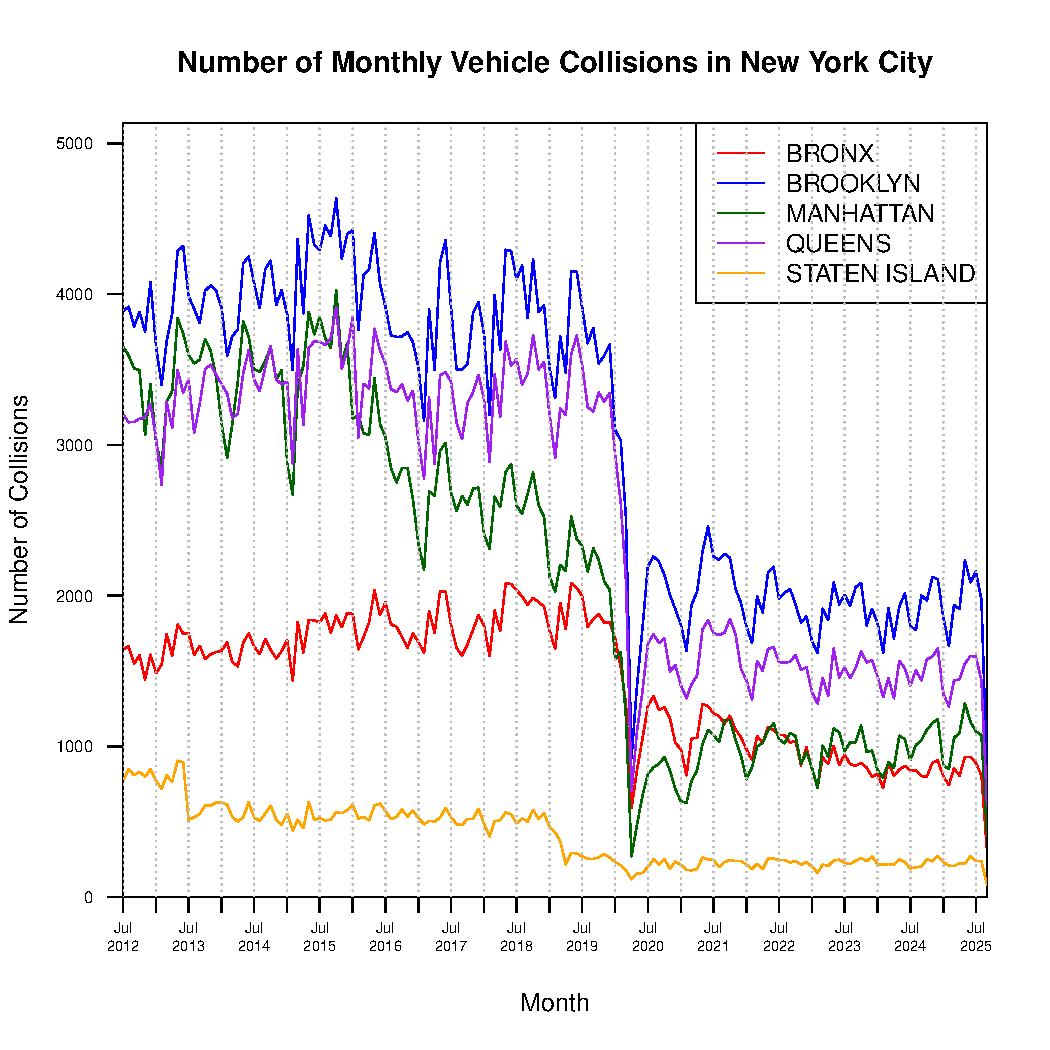
\includegraphics[width=\maxwidth]{figure/unnamed-chunk-3-1} 
\end{knitrout}
Each borough follows very similar shapes in their respective line. Further analysis to normalize by some factor, e.g. by population or road network density may provide more insight.

\subsection{Causes of Collisions}
In the dataset every entry has up to 5 `contributing factors'. Below, We see these results aggregated and the top 5 most prevalent causes displayed in a bar chart.
\begin{knitrout}
\definecolor{shadecolor}{rgb}{0.969, 0.969, 0.969}\color{fgcolor}\begin{kframe}
\begin{alltt}
\hldef{cfs} \hlkwb{<-} \hlkwd{unique}\hldef{(nyc}\hlopt{$}\hldef{CONTRIBUTING.FACTOR.VEHICLE.1)}
\hldef{cont_fact} \hlkwb{<-} \hlkwd{c}\hldef{()}
\hlkwa{for} \hldef{(f} \hlkwa{in} \hldef{cfs)\{}
  \hldef{s} \hlkwb{<-} \hlnum{0}
  \hlkwa{for} \hldef{(i} \hlkwa{in} \hlnum{1}\hlopt{:}\hlnum{5}\hldef{)\{}
    \hldef{colmn} \hlkwb{<-} \hlkwd{paste0}\hldef{(}\hlsng{"CONTRIBUTING.FACTOR.VEHICLE."}\hldef{,i)}
    \hldef{s} \hlkwb{<-} \hldef{s} \hlopt{+} \hlkwd{sum}\hldef{(nyc[[colmn]]} \hlopt{==} \hldef{f)}
  \hldef{\}}
  \hldef{cont_fact} \hlkwb{<-} \hlkwd{append}\hldef{(cont_fact,s)}
\hldef{\}}
\hlkwd{names}\hldef{(cont_fact)} \hlkwb{<-} \hldef{cfs}
\hldef{fivemost} \hlkwb{<-} \hlkwd{sort}\hldef{(cont_fact,} \hlkwc{decreasing}\hldef{=}\hlnum{TRUE}\hldef{)[}\hlnum{3}\hlopt{:}\hlnum{7}\hldef{]}
\hlcom{#1st and 2nd are unspecified or null}

\hlkwd{par}\hldef{(}\hlkwc{mar} \hldef{=} \hlkwd{c}\hldef{(}\hlnum{10}\hldef{,} \hlnum{5}\hldef{,} \hlnum{4}\hldef{,} \hlnum{2}\hldef{))}
\hlkwd{barplot}\hldef{(fivemost,}
        \hlkwc{main} \hldef{=} \hlsng{"Top Contributing Factors"}\hldef{,}
        \hlkwc{col} \hldef{=} \hlkwd{c}\hldef{(}\hlsng{"darkseagreen4"}\hldef{,} \hlsng{"darkseagreen"}\hldef{,} \hlsng{"darkseagreen3"}\hldef{,}
                \hlsng{"darkseagreen2"}\hldef{,} \hlsng{"darkseagreen1"}\hldef{),}
        \hlkwc{las} \hldef{=} \hlnum{2}\hldef{,}
        \hlkwc{cex.names} \hldef{=} \hlnum{0.8}\hldef{,}
        \hlkwc{yaxt} \hldef{=} \hlsng{"n"}\hldef{,}
        \hlkwc{ylim} \hldef{=} \hlkwd{c}\hldef{(}\hlnum{0}\hldef{,}\hlkwd{ceiling}\hldef{(}\hlkwd{max}\hldef{(fivemost)}\hlopt{/}\hlnum{100000}\hldef{)}\hlopt{*}\hlnum{100000}\hldef{)}
        \hldef{)}

\hlkwd{title}\hldef{(}\hlkwc{ylab} \hldef{=} \hlsng{"Number of Cases"}\hldef{,} \hlkwc{line}\hldef{=}\hlnum{4}\hldef{)}

\hlkwd{axis}\hldef{(}\hlnum{2}\hldef{,} \hlkwc{at} \hldef{=} \hlkwd{seq}\hldef{(}\hlnum{0}\hldef{,} \hlkwd{ceiling}\hldef{(}\hlkwd{max}\hldef{(fivemost)}\hlopt{/}\hlnum{100000}\hldef{)}\hlopt{*}\hlnum{100000}\hldef{,} \hlkwc{by} \hldef{=} \hlnum{100000}\hldef{),}
     \hlkwc{labels} \hldef{=} \hlkwd{format}\hldef{(}\hlkwd{seq}\hldef{(}\hlnum{0}\hldef{,} \hlkwd{ceiling}\hldef{(}\hlkwd{max}\hldef{(fivemost)}\hlopt{/}\hlnum{100000}\hldef{)}\hlopt{*}\hlnum{100000}\hldef{,} \hlkwc{by} \hldef{=} \hlnum{100000}\hldef{),}
                     \hlkwc{big.mark} \hldef{=} \hlsng{","}\hldef{,}
                     \hlkwc{scientific} \hldef{=} \hlnum{FALSE}\hldef{),}
     \hlkwc{cex.axis} \hldef{=} \hlnum{0.8}\hldef{,}
     \hlkwc{las} \hldef{=} \hlnum{1}\hldef{,}
     \hldef{)}
\end{alltt}
\end{kframe}
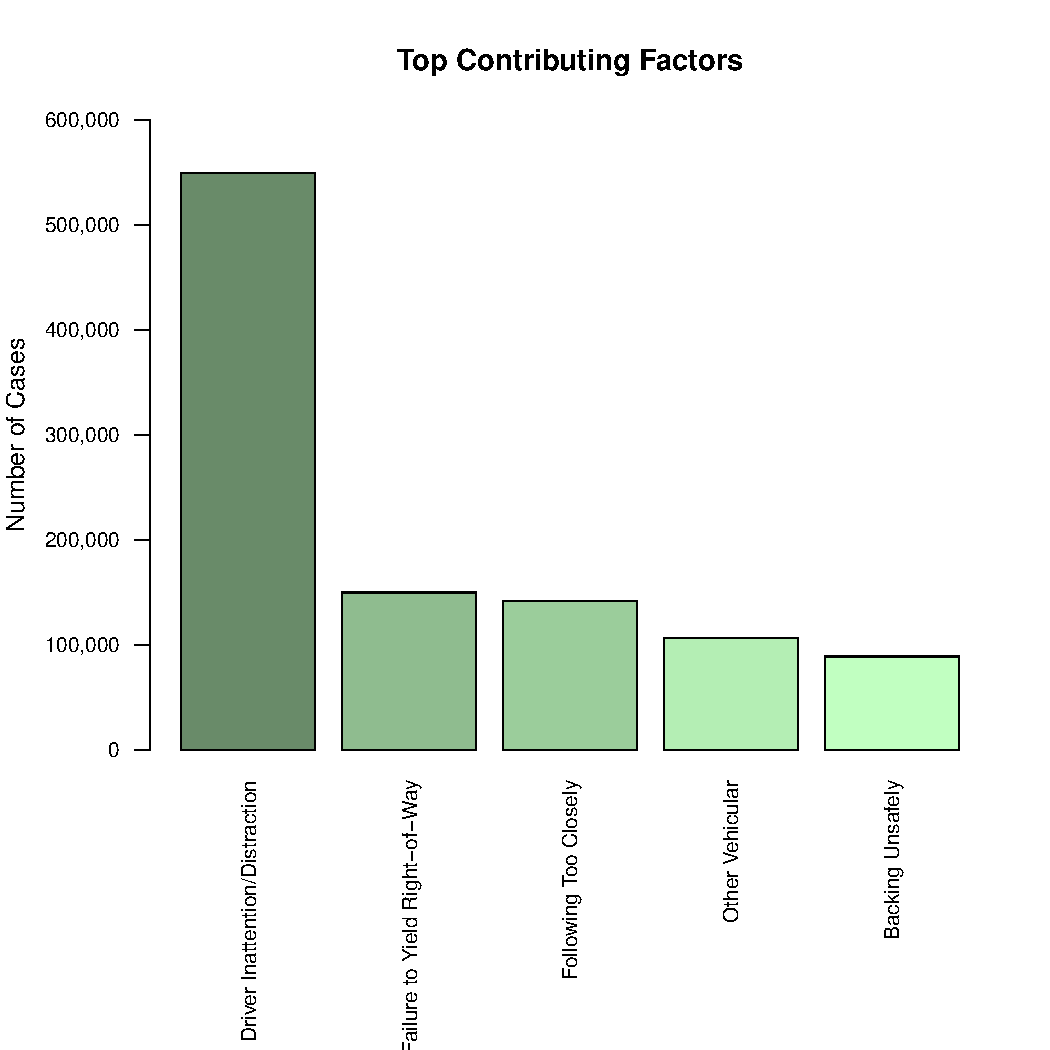
\includegraphics[width=\maxwidth]{figure/unnamed-chunk-4-1} 
\end{knitrout}
An overwhelming cause of accidents are due to driver distraction, more than 3 times the next most common.


\subsection{Crashes by Time of Day}

The histogram below shows the total number of accidents in the dataset for each time of day. 

\begin{knitrout}
\definecolor{shadecolor}{rgb}{0.969, 0.969, 0.969}\color{fgcolor}\begin{kframe}
\begin{alltt}
\hlkwd{layout}\hldef{(}\hlkwc{mat} \hldef{=} \hlnum{1}\hldef{)}
\hldef{times} \hlkwb{<-} \hldef{nyc}\hlopt{$}\hldef{CRASH.TIME}
\hldef{hours} \hlkwb{<-} \hlkwd{as.numeric}\hldef{(}\hlkwd{sub}\hldef{(}\hlsng{"\textbackslash{}\textbackslash{}:.*"}\hldef{,} \hlsng{""}\hldef{, times))}
\hlkwd{par}\hldef{(}\hlkwc{tck} \hldef{=} \hlopt{-}\hlnum{0.015}\hldef{,} \hlkwc{mgp} \hldef{=} \hlkwd{c}\hldef{(}\hlnum{1.5}\hldef{,} \hlnum{0.4}\hldef{,} \hlnum{0}\hldef{),} \hlkwc{mar} \hldef{=} \hlkwd{c}\hldef{(}\hlnum{3}\hldef{,} \hlnum{3}\hldef{,} \hlnum{3}\hldef{,} \hlnum{1.5}\hldef{))}
\hlkwd{hist}\hldef{(hours,} \hlkwc{xlab} \hldef{=} \hlsng{"Time of day"}\hldef{,} \hlkwc{ylab} \hldef{=} \hlsng{"Number of accidents"}\hldef{,} \hlkwc{axes} \hldef{=} \hlnum{FALSE}\hldef{,}
     \hlkwc{main}\hldef{=}\hlsng{"Total Number of Accidents per Time of Day"}\hldef{,}
     \hlkwc{breaks}\hldef{=}\hlkwd{seq}\hldef{(}\hlopt{-}\hlnum{0.5}\hldef{,} \hlnum{23.5}\hldef{,} \hlnum{1}\hldef{))}

\hldef{labels} \hlkwb{<-} \hlkwd{c}\hldef{(}\hlsng{"12:00AM"}\hldef{,} \hlsng{"3:00AM"}\hldef{,} \hlsng{"6:00AM"}\hldef{,} \hlsng{"9:00AM"}\hldef{,}
            \hlsng{"12:00PM"}\hldef{,} \hlsng{"3:00PM"}\hldef{,} \hlsng{"6:00PM"}\hldef{,} \hlsng{"9:00PM"}\hldef{)}
\hldef{axp} \hlkwb{<-} \hlkwd{seq}\hldef{(}\hlnum{0}\hldef{,} \hlnum{23}\hldef{,} \hlkwc{by}\hldef{=}\hlnum{3}\hldef{)}
\hlkwd{axis}\hldef{(}\hlnum{1}\hldef{,} \hlkwc{at}\hldef{=axp,} \hlkwc{labels} \hldef{= labels)}
\hldef{axp2} \hlkwb{<-} \hlkwd{seq}\hldef{(}\hlnum{0}\hldef{,} \hlnum{150000}\hldef{,} \hlkwc{by}\hldef{=}\hlnum{50000}\hldef{)}
\hlkwd{axis}\hldef{(}\hlnum{2}\hldef{,} \hlkwc{at} \hldef{= axp2,} \hlkwc{labels} \hldef{= axp2)}
\end{alltt}
\end{kframe}
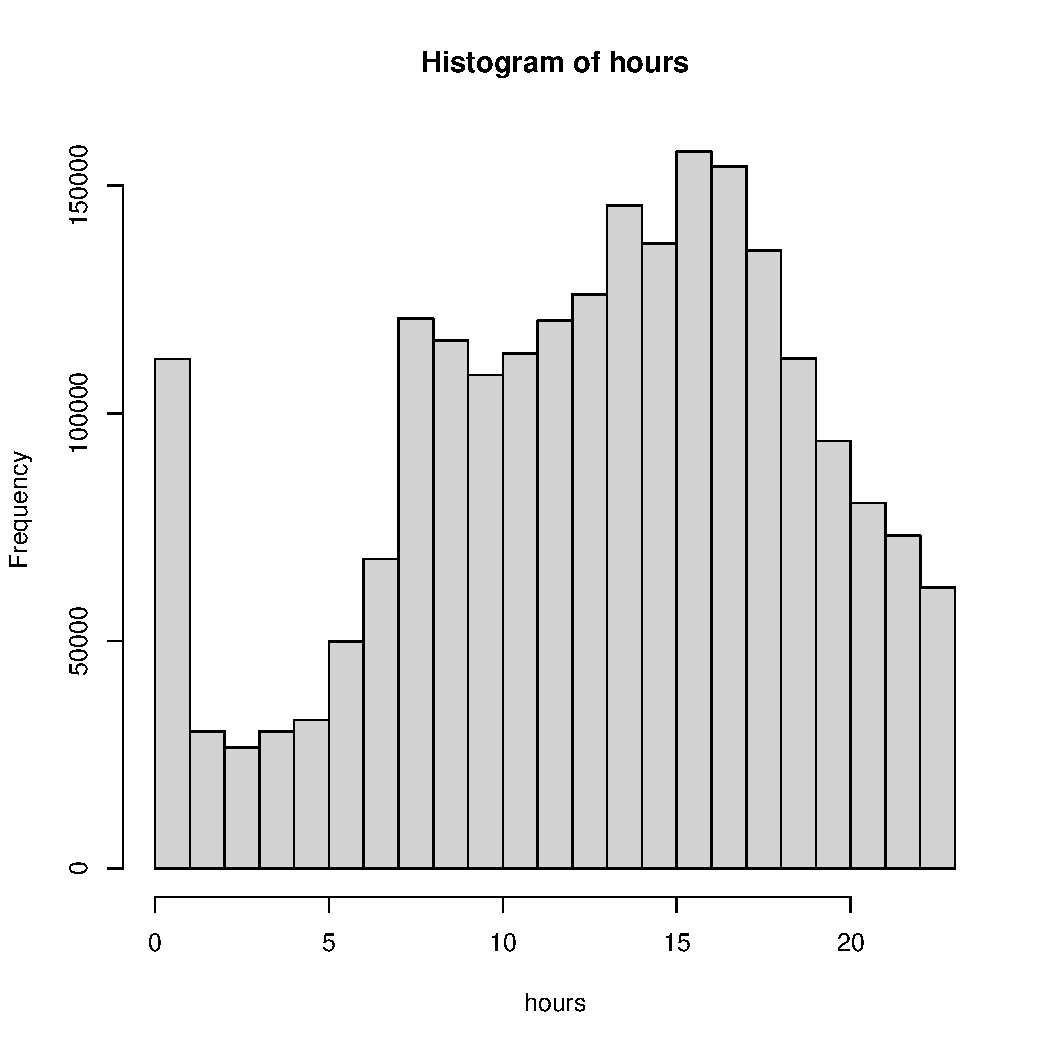
\includegraphics[width=\maxwidth]{figure/unnamed-chunk-5-1} 
\end{knitrout}

We can see that most of the accidents occur during the daytime, with a semi-continuous increasing and decreasing structure. The distribution reaches its lowest value at 3:00AM, and peaks around 4:00PM. There are slight spikes around 8-9AM, when people would be driving to work, and also around 4-5:00PM, when people would be leaving work. There is also a small spike around midnight.

\subsection{Injuries by Person Type}

This series of box plots focuses on collisions that resulted in at least 10 total injuries. We compare the total number of people injured with the amounts of people injured of different types: pedestrians, motorists, and cyclists.

\begin{knitrout}
\definecolor{shadecolor}{rgb}{0.969, 0.969, 0.969}\color{fgcolor}\begin{kframe}
\begin{alltt}
\hldef{people_injured} \hlkwb{<-} \hldef{nyc}\hlopt{$}\hldef{NUMBER.OF.PERSONS.INJURED}
\hldef{pedestrians_injured} \hlkwb{<-} \hldef{nyc}\hlopt{$}\hldef{NUMBER.OF.PEDESTRIANS.INJURED}
\hldef{motorists_injured} \hlkwb{<-} \hldef{nyc}\hlopt{$}\hldef{NUMBER.OF.MOTORIST.INJURED}
\hldef{cyclists_injured} \hlkwb{<-} \hldef{nyc}\hlopt{$}\hldef{NUMBER.OF.CYCLIST.INJURED}

\hldef{mass_factor} \hlkwb{<-} \hldef{people_injured} \hlopt{>=} \hlnum{10}
\hldef{people_injured_mass} \hlkwb{<-} \hldef{people_injured[mass_factor]}
\hldef{motorists_injured_mass} \hlkwb{<-} \hldef{motorists_injured[mass_factor]}
\hldef{pedestrians_injured_mass} \hlkwb{<-} \hldef{pedestrians_injured[mass_factor]}
\hldef{cyclists_injured_mass} \hlkwb{<-} \hldef{cyclists_injured[mass_factor]}
\hlkwd{layout}\hldef{(}\hlkwc{mat} \hldef{=} \hlkwd{matrix}\hldef{(}\hlkwd{c}\hldef{(}\hlnum{1}\hldef{,} \hlnum{2}\hldef{,} \hlnum{3}\hldef{,} \hlnum{4}\hldef{),} \hlnum{4}\hldef{,} \hlkwc{byrow} \hldef{=} \hlnum{TRUE}\hldef{))}
\hlkwd{boxplot}\hldef{(people_injured_mass,}
        \hlkwc{main}\hldef{=}\hlsng{"total people injured for mass casualty events 
        (over 10 people injured)"}\hldef{,}
        \hlkwc{horizontal}\hldef{=}\hlnum{TRUE}\hldef{,} \hlkwc{ylim} \hldef{=} \hlkwd{c}\hldef{(}\hlnum{0}\hldef{,} \hlnum{45}\hldef{))}
\hlkwd{boxplot}\hldef{(motorists_injured_mass,} \hlkwc{main}\hldef{=}\hlsng{"motorists injured"}\hldef{,}
        \hlkwc{horizontal}\hldef{=}\hlnum{TRUE}\hldef{,} \hlkwc{ylim} \hldef{=} \hlkwd{c}\hldef{(}\hlnum{0}\hldef{,} \hlnum{45}\hldef{))}
\hlkwd{boxplot}\hldef{(pedestrians_injured_mass,} \hlkwc{main}\hldef{=}\hlsng{"pedestrians injured"}\hldef{,}
        \hlkwc{horizontal}\hldef{=}\hlnum{TRUE}\hldef{,} \hlkwc{ylim} \hldef{=} \hlkwd{c}\hldef{(}\hlnum{0}\hldef{,} \hlnum{45}\hldef{))}
\hlkwd{boxplot}\hldef{(cyclists_injured_mass,} \hlkwc{main} \hldef{=} \hlsng{"cyclists injured"}\hldef{,}
        \hlkwc{horizontal}\hldef{=}\hlnum{TRUE}\hldef{,} \hlkwc{ylim} \hldef{=} \hlkwd{c}\hldef{(}\hlnum{0}\hldef{,} \hlnum{45}\hldef{))}
\end{alltt}
\end{kframe}
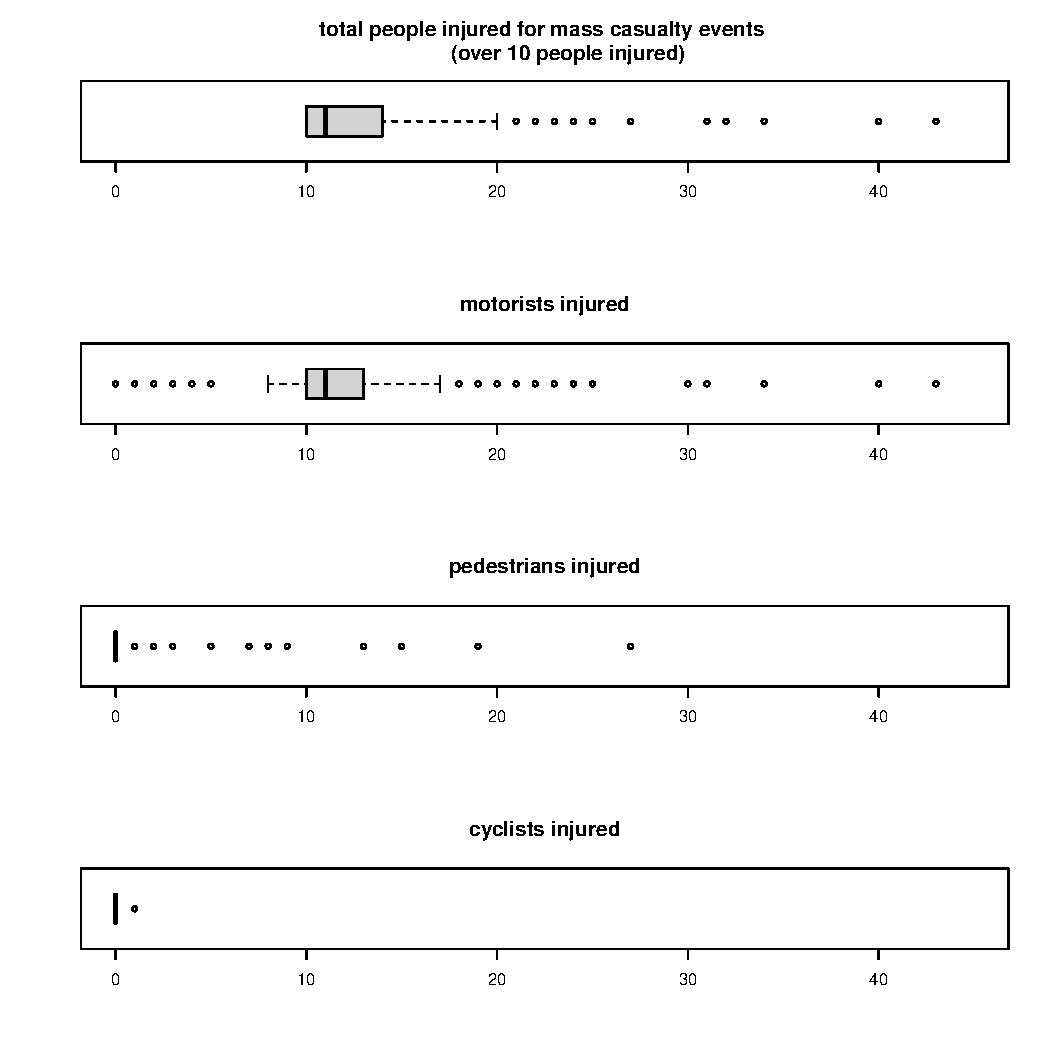
\includegraphics[width=\maxwidth]{figure/unnamed-chunk-6-1} 
\end{knitrout}

The vast majority of these collisions resulted in motorists being the main affected group. This is unsurprising, as every collision must involve motorists, but the other possible parties may not even be present. Pedestrians were mostly uninjured by these collisions, with some exceptions that result in the amount of pedestrian injuries to go into the 20s. Cyclists were the most unaffected by these mass injury collisions, with a couple of collisions injuring one cyclist, but otherwise 0 cyclists were injured in any of the other collisions. 


\subsection{Borough VS Injury Severity}

\subsubsection{Contingency Table}

This contingency table examines whether crash severity (fatal, injury, or no injury) varies across NYC boroughs.

\begin{knitrout}
\definecolor{shadecolor}{rgb}{0.969, 0.969, 0.969}\color{fgcolor}\begin{kframe}
\begin{alltt}
\hldef{nyc}\hlopt{$}\hldef{injury_severity} \hlkwb{<-} \hlkwd{ifelse}\hldef{(nyc}\hlopt{$}\hldef{NUMBER.OF.CYCLIST.KILLED} \hlopt{>} \hlnum{0}\hldef{,}
                              \hlsng{"FATAL/DIED"}\hldef{,}
                       \hlkwd{ifelse}\hldef{(nyc}\hlopt{$}\hldef{NUMBER.OF.PERSONS.INJURED} \hlopt{>} \hlnum{0}\hldef{,}
                              \hlsng{"INJURY"}\hldef{,} \hlsng{"NO INJURY"}\hldef{))}


\hlcom{# removing NA's}
\hldef{borough_injury_data} \hlkwb{<-} \hldef{nyc[}\hlopt{!}\hlkwd{is.na}\hldef{(nyc}\hlopt{$}\hldef{BOROUGH)} \hlopt{& !}\hlkwd{is.na}\hldef{(nyc}\hlopt{$}\hldef{injury_severity), ]}

\hlcom{# Contingency Table}
\hldef{(borough_injury_table} \hlkwb{<-} \hlkwd{table}\hldef{(borough_injury_data}\hlopt{$}\hldef{BOROUGH,}
                               \hldef{borough_injury_data}\hlopt{$}\hldef{injury_severity))}
\end{alltt}
\begin{verbatim}
##                
##                 FATAL/DIED INJURY NO INJURY
##                         75 170997    506210
##   BRONX                 30  57186    169143
##   BROOKLYN              75 127827    361518
##   MANHATTAN             48  64000    274797
##   QUEENS                40  97339    312283
##   STATEN ISLAND          4  14005     50023
\end{verbatim}
\end{kframe}
\end{knitrout}

\begin{knitrout}
\definecolor{shadecolor}{rgb}{0.969, 0.969, 0.969}\color{fgcolor}\begin{kframe}
\begin{alltt}
\hlcom{# Chi-square test}
\hldef{(chi_test1} \hlkwb{<-} \hlkwd{chisq.test}\hldef{(borough_injury_table))}
\end{alltt}
\begin{verbatim}
## 
## 	Pearson's Chi-squared test
## 
## data:  borough_injury_table
## X-squared = 6988.6, df = 10, p-value < 2.2e-16
\end{verbatim}
\end{kframe}
\end{knitrout}

Since p-value < alpha = 0.05, we reject the null hypothesis and conclude that we have sufficient evidence to prove the true population of boroughs are not evenly distributed or in other words, that the distribution of fatal, injury, and property-damage-only crashes varies significantly across NYC boroughs (Chi-square, df=8, p-value < 0.0001). Furthermore, there is a massive test statistic of $X^2$ = 6377.3 which shows the huge differences between what we'd expect if boroughs were all the same vs. what we actually observe.


\subsubsection{Barplot of Row Proportions (by Borough)}
This barplot shows crash severity proportions within each borough.

\begin{knitrout}
\definecolor{shadecolor}{rgb}{0.969, 0.969, 0.969}\color{fgcolor}\begin{kframe}
\begin{alltt}
\hldef{(prop_table1} \hlkwb{<-} \hlkwd{prop.table}\hldef{(borough_injury_table,} \hlkwc{margin} \hldef{=} \hlnum{1}\hldef{))}
\end{alltt}
\begin{verbatim}
##                
##                   FATAL/DIED       INJURY    NO INJURY
##                 1.107367e-04 2.524753e-01 7.474139e-01
##   BRONX         1.325328e-04 2.526341e-01 7.472334e-01
##   BROOKLYN      1.532426e-04 2.611806e-01 7.386662e-01
##   MANHATTAN     1.416577e-04 1.888769e-01 8.109814e-01
##   QUEENS        9.764147e-05 2.376081e-01 7.622943e-01
##   STATEN ISLAND 6.246877e-05 2.187188e-01 7.812188e-01
\end{verbatim}
\begin{alltt}
\hlkwd{barplot}\hldef{(prop_table1)}
\end{alltt}
\end{kframe}
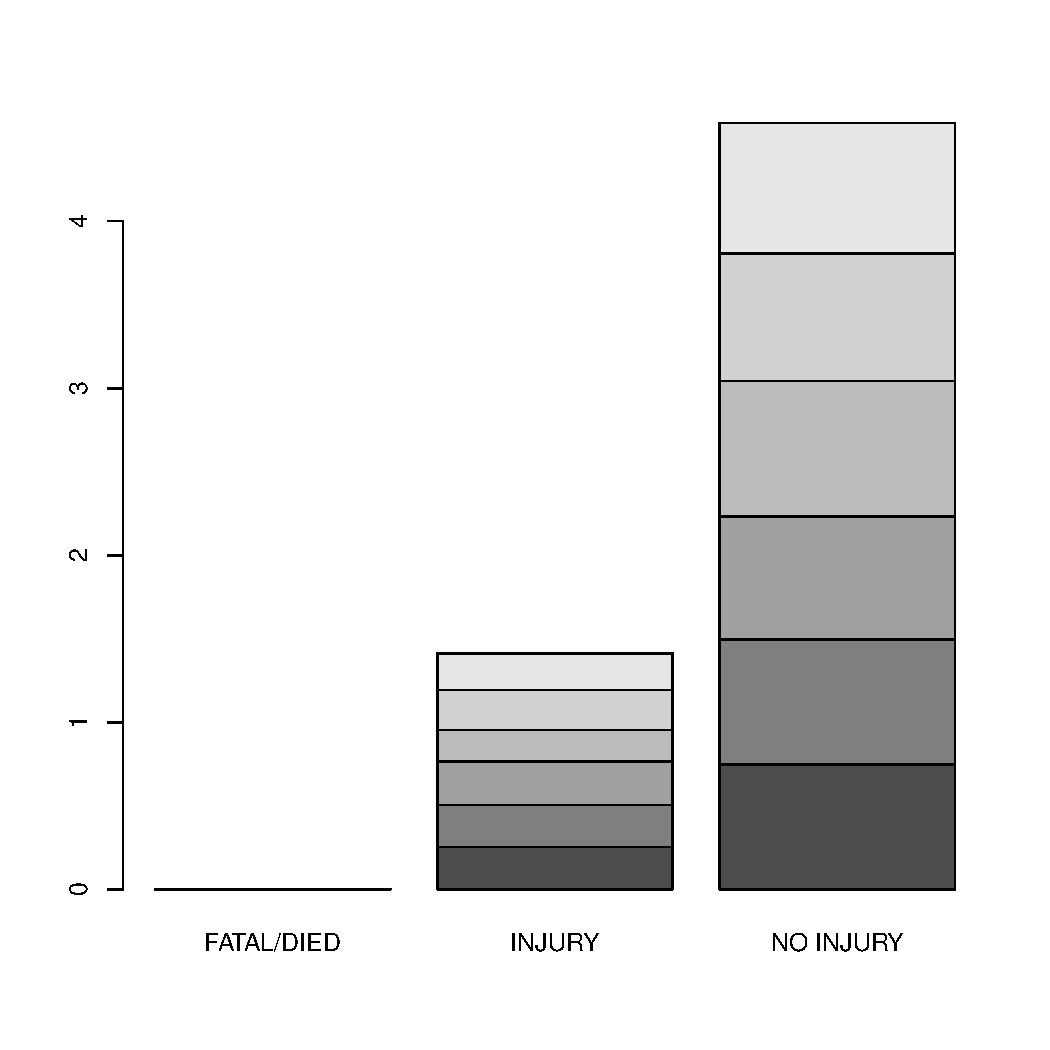
\includegraphics[width=\maxwidth]{figure/unnamed-chunk-9-1} 
\end{knitrout}

While all boroughs have low fatal crash rates (around 0.1-0.16\%), Staten Island has the highest fatality rate at 0.159\%, followed by Brooklyn at 0.142\%. Manhattan appears to be the safest borough with the lowest rates of both fatal (0.107\%) and injury crashes (18.9\%). Brooklyn and the Bronx have the highest injury rates at 26.1\% and 25.3\% respectively, while Manhattan has significantly more no injury crashes (80.1\%) compared to other boroughs.

\subsubsection{Cramer’s V}



\begin{knitrout}
\definecolor{shadecolor}{rgb}{0.969, 0.969, 0.969}\color{fgcolor}\begin{kframe}
\begin{alltt}
\hlkwd{cramerV}\hldef{(borough_injury_table)}
\end{alltt}
\begin{verbatim}
## Cramer V 
##   0.0398
\end{verbatim}
\end{kframe}
\end{knitrout}

The chi-square test concluded that there is a statistically significant association between borough and crash severity. However, the effect size was very small (Cramer's V = 0.046), indicating that while borough differences are statistically detectable, they explain less than 1\% of the variation in crash severity. This suggests that factors other than borough location are much more important in determining crash outcomes.

\subsection{Total Persons Injured vs Killed}
This scatterplot examines the relationship between injuries and fatalities in NYC vehicle crashes.
\begin{knitrout}
\definecolor{shadecolor}{rgb}{0.969, 0.969, 0.969}\color{fgcolor}\begin{kframe}
\begin{alltt}
\hldef{injury_data} \hlkwb{<-} \hldef{nyc[nyc}\hlopt{$}\hldef{NUMBER.OF.PERSONS.INJURED} \hlopt{>} \hlnum{0} \hlopt{|}
                     \hldef{nyc}\hlopt{$}\hldef{NUMBER.OF.PERSONS.KILLED} \hlopt{>} \hlnum{0}\hldef{, ]}

\hlkwd{plot}\hldef{(injury_data}\hlopt{$}\hldef{NUMBER.OF.PERSONS.INJURED,}
     \hldef{injury_data}\hlopt{$}\hldef{NUMBER.OF.PERSONS.KILLED,}
     \hlkwc{main} \hldef{=} \hlsng{"Relationship Between Injuries and Fatalities in NYC Crashes"}\hldef{,}
     \hlkwc{xlab} \hldef{=} \hlsng{"Number of Persons Injured"}\hldef{,}
     \hlkwc{ylab} \hldef{=} \hlsng{"Number of Persons Killed"}\hldef{,}
     \hlkwc{pch} \hldef{=} \hlnum{16}\hldef{,}
     \hlkwc{col} \hldef{=} \hlsng{"darkblue"}\hldef{,}
     \hlkwc{cex} \hldef{=} \hlnum{0.6}\hldef{)}

\hlkwd{abline}\hldef{(}\hlkwd{lm}\hldef{(injury_data}\hlopt{$}\hldef{NUMBER.OF.PERSONS.KILLED} \hlopt{~}
            \hldef{injury_data}\hlopt{$}\hldef{NUMBER.OF.PERSONS.INJURED),}
       \hlkwc{col} \hldef{=} \hlsng{"red"}\hldef{,} \hlkwc{lwd} \hldef{=} \hlnum{2}\hldef{)}
\end{alltt}
\end{kframe}
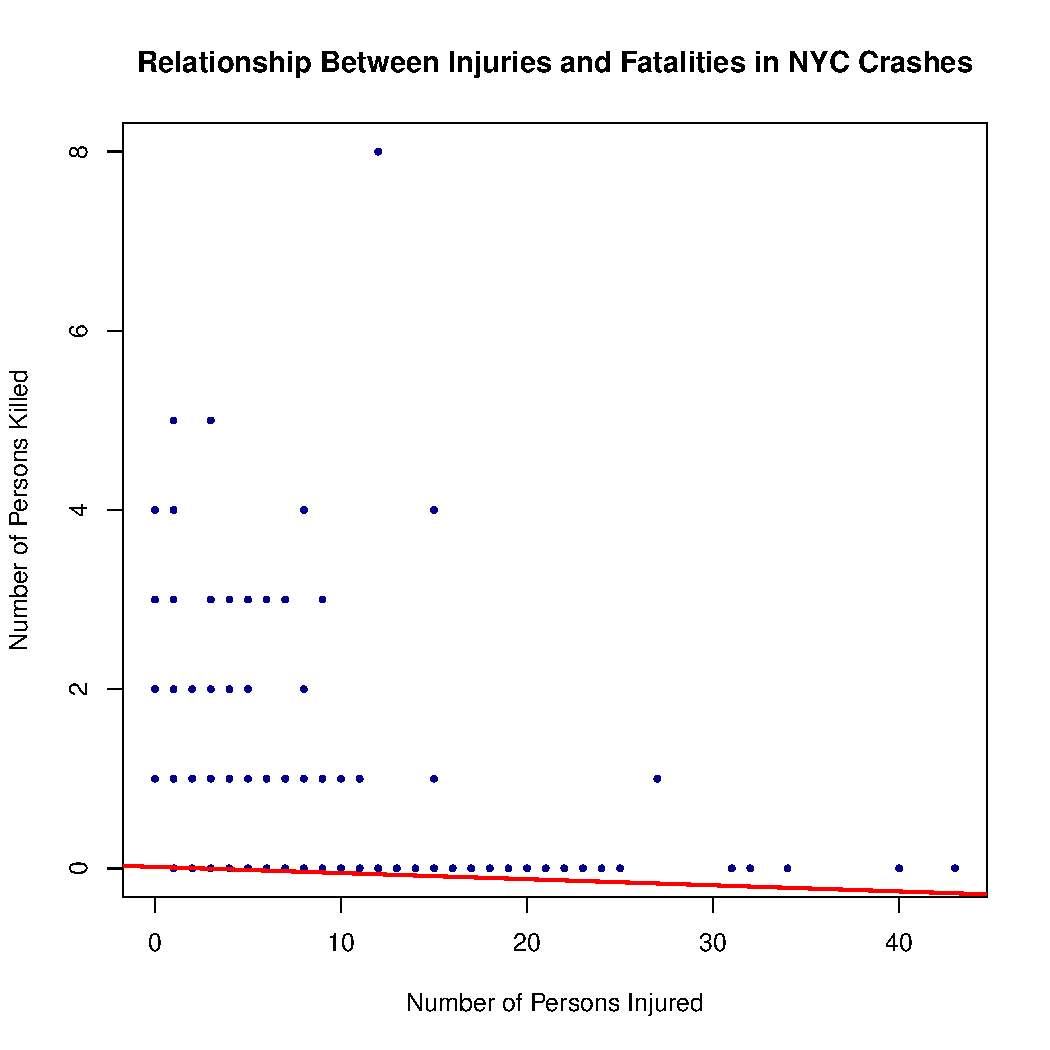
\includegraphics[width=\maxwidth]{figure/unnamed-chunk-12-1} 
\end{knitrout}

The plot shows that most crashes result in injuries but no deaths which can be seen by the concentration of points along the bottom. Fatal crashes are rare and scattered across injury levels, with no clear correlation. The flat regression line shows that there is a minimal relationship between injuries and deaths, suggesting fatalities depend more on crash circumstances than the number of people involved.



\section{Preliminary Statistical Modeling \& Interpretation}

To better understand the factors that influence the severity of motor vehicle collisions in New York City, we developed a preliminary statistical model using logistic regression. The outcome of interest is whether a crash was fatal (at least one person killed) or non-fatal. Logistic regression is appropriate in this context because the outcome is binary (fatal vs. non-fatal), and it allows us to estimate how different factors change the odds of a fatal crash while holding other conditions constant.

The predictors included in the model were the borough of occurrence, time of day (day vs. night), vehicle type, and the primary contributing factor reported by police. By examining the estimated odds ratios and their statistical significance, we can identify which circumstances or behaviors are most strongly associated with fatal outcomes.

\subsection{Code and Results}



Data cleansing and transformations:
\begin{knitrout}
\definecolor{shadecolor}{rgb}{0.969, 0.969, 0.969}\color{fgcolor}\begin{kframe}
\begin{alltt}
\hldef{nyc_small} \hlkwb{<-} \hldef{nyc} \hlopt
  \hlkwd{filter}\hldef{(BOROUGH} \hlopt{!=} \hlsng{""} \hlopt{&}
           \hldef{CONTRIBUTING.FACTOR.VEHICLE.1} \hlopt{!=} \hlsng{""} \hlopt{&}
           \hldef{CONTRIBUTING.FACTOR.VEHICLE.1} \hlopt{!=} \hlsng{"1"} \hlopt{&}
           \hldef{CONTRIBUTING.FACTOR.VEHICLE.1} \hlopt{!=} \hlsng{"80"}\hldef{)} \hlopt
  \hlkwd{transmute}\hldef{(}
    \hlkwc{is_fatal} \hldef{=} \hlkwd{ifelse}\hldef{(NUMBER.OF.PERSONS.KILLED} \hlopt{>} \hlnum{0}\hldef{,} \hlnum{1}\hldef{,} \hlnum{0}\hldef{),}  \hlcom{# outcome}
    \hlkwc{borough} \hldef{= BOROUGH,}
    \hlkwc{crash_hour} \hldef{=} \hlkwd{hour}\hldef{(}\hlkwd{hm}\hldef{(CRASH.TIME)),}
    \hlkwc{contributing_factor} \hldef{= CONTRIBUTING.FACTOR.VEHICLE.1,}
    \hlkwc{vehicle_cat} \hldef{=} \hlkwd{factor}\hldef{(}\hlkwd{case_when}\hldef{(}
      \hlkwd{grepl}\hldef{(}\hlsng{"MOTORCYCLE|MOTORBIKE"}\hldef{, VEHICLE.TYPE.CODE.1,} \hlkwc{ignore.case} \hldef{=} \hlnum{TRUE}\hldef{)} \hlopt{~}
        \hlsng{"motorcycle"}\hldef{,}
      \hlkwd{grepl}\hldef{(}\hlsng{"TRUCK|BUS"}\hldef{, VEHICLE.TYPE.CODE.1,} \hlkwc{ignore.case} \hldef{=} \hlnum{TRUE}\hldef{)} \hlopt{~}
        \hlsng{"truck_bus"}\hldef{,}
      \hlkwd{grepl}\hldef{(}\hlsng{"BICYCLE|BIKE|SCOOTER"}\hldef{, VEHICLE.TYPE.CODE.1,} \hlkwc{ignore.case} \hldef{=} \hlnum{TRUE}\hldef{)} \hlopt{~}
        \hlsng{"bike_scooter"}\hldef{,}
      \hlnum{TRUE} \hlopt{~} \hlsng{"car_suv"}
    \hldef{))}
  \hldef{)}

\hldef{nyc_small} \hlkwb{<-} \hldef{nyc_small} \hlopt
  \hlkwd{mutate}\hldef{(}\hlkwc{hour} \hldef{=} \hlkwd{as.numeric}\hldef{(}\hlkwd{substr}\hldef{(crash_hour,} \hlnum{1}\hldef{,} \hlnum{2}\hldef{)),}
         \hlkwc{tod} \hldef{=} \hlkwd{ifelse}\hldef{(hour} \hlopt{>=} \hlnum{6} \hlopt{&} \hldef{hour} \hlopt{<} \hlnum{18}\hldef{,} \hlsng{"day"}\hldef{,} \hlsng{"night"}\hldef{))}

\hldef{nyc_small}\hlopt{$}\hldef{BOROUGH} \hlkwb{<-} \hlkwd{droplevels}\hldef{(}\hlkwd{as.factor}\hldef{(nyc_small}\hlopt{$}\hldef{borough))}

\hlcom{# set baselines for model}
\hldef{nyc_small}\hlopt{$}\hldef{borough} \hlkwb{<-} \hlkwd{relevel}\hldef{(}\hlkwd{as.factor}\hldef{(nyc_small}\hlopt{$}\hldef{BOROUGH),}
                             \hlkwc{ref} \hldef{=} \hlsng{"STATEN ISLAND"}\hldef{)}
\hldef{nyc_small}\hlopt{$}\hldef{tod} \hlkwb{<-} \hlkwd{relevel}\hldef{(}\hlkwd{as.factor}\hldef{(nyc_small}\hlopt{$}\hldef{tod),}
                         \hlkwc{ref} \hldef{=} \hlsng{"day"}\hldef{)}
\hldef{nyc_small}\hlopt{$}\hldef{vehicle_cat} \hlkwb{<-} \hlkwd{relevel}\hldef{(}\hlkwd{as.factor}\hldef{(nyc_small}\hlopt{$}\hldef{vehicle_cat),}
                                 \hlkwc{ref} \hldef{=} \hlsng{"car_suv"}\hldef{)}
\hldef{nyc_small}\hlopt{$}\hldef{contributing_factor} \hlkwb{<-} \hlkwd{relevel}\hldef{(}
  \hlkwd{as.factor}\hldef{(nyc_small}\hlopt{$}\hldef{contributing_factor),}\hlkwc{ref} \hldef{=} \hlsng{"Unspecified"}\hldef{)}
\end{alltt}
\end{kframe}
\end{knitrout}

Creating the logistic regression model:
\begin{knitrout}
\definecolor{shadecolor}{rgb}{0.969, 0.969, 0.969}\color{fgcolor}\begin{kframe}
\begin{alltt}
\hldef{model} \hlkwb{<-} \hlkwd{glm}\hldef{(is_fatal} \hlopt{~} \hldef{borough} \hlopt{+} \hldef{tod} \hlopt{+} \hldef{vehicle_cat} \hlopt{+} \hldef{contributing_factor,}
             \hlkwc{data} \hldef{= nyc_small,}
             \hlkwc{family} \hldef{= binomial)}


\hldef{summ} \hlkwb{<-} \hlkwd{summary}\hldef{(model)}

\hldef{coefs} \hlkwb{<-} \hldef{summ}\hlopt{$}\hldef{coefficients}
\hldef{est} \hlkwb{<-} \hldef{coefs[,} \hlsng{"Estimate"}\hldef{]}         \hlcom{# log-odds}
\hldef{se}  \hlkwb{<-} \hldef{coefs[,} \hlsng{"Std. Error"}\hldef{]}       \hlcom{# standard errors}

\hlcom{# compute odds ratios + 95% confidence intervals}
\hldef{ci_low}  \hlkwb{<-} \hlkwd{exp}\hldef{(est} \hlopt{-} \hlnum{1.96} \hlopt{*} \hldef{se)}
\hldef{ci_high} \hlkwb{<-} \hlkwd{exp}\hldef{(est} \hlopt{+} \hlnum{1.96} \hlopt{*} \hldef{se)}

\hldef{results_table} \hlkwb{<-} \hlkwd{data.frame}\hldef{(}
  \hlkwc{term}        \hldef{=} \hlkwd{rownames}\hldef{(coefs),}
  \hlkwc{odds_ratio}  \hldef{=} \hlkwd{exp}\hldef{(est),}
  \hlkwc{ci_low}      \hldef{= ci_low,}
  \hlkwc{ci_high}     \hldef{= ci_high,}
  \hlkwc{significant} \hldef{=} \hlkwd{ifelse}\hldef{(coefs[,} \hlsng{"Pr(>|z|)"}\hldef{]} \hlopt{<} \hlnum{0.05}\hldef{,} \hlsng{"yes"}\hldef{,} \hlsng{"no"}\hldef{),}
  \hlkwc{row.names}   \hldef{=} \hlkwa{NULL}
\hldef{)}

\hlcom{# filter out the intercept/baseline to keep table cleaner}
\hldef{results_table} \hlkwb{<-} \hldef{results_table[results_table}\hlopt{$}\hldef{term} \hlopt{!=} \hlsng{"(Intercept)"}\hldef{, ]}

\hldef{results_table}\hlopt{$}\hldef{term} \hlkwb{<-} \hlkwd{gsub}\hldef{(}\hlsng{"vehicle_cat"}\hldef{,} \hlsng{"Vehicle: "}\hldef{,}
                           \hldef{results_table}\hlopt{$}\hldef{term)}
\hldef{results_table}\hlopt{$}\hldef{term} \hlkwb{<-} \hlkwd{gsub}\hldef{(}\hlsng{"borough"}\hldef{,} \hlsng{"Borough: "}\hldef{,}
                           \hldef{results_table}\hlopt{$}\hldef{term)}
\hldef{results_table}\hlopt{$}\hldef{term} \hlkwb{<-} \hlkwd{gsub}\hldef{(}\hlsng{"tod"}\hldef{,} \hlsng{"Time of Day: "}\hldef{,}
                           \hldef{results_table}\hlopt{$}\hldef{term)}
\hldef{results_table}\hlopt{$}\hldef{term} \hlkwb{<-} \hlkwd{gsub}\hldef{(}\hlsng{"contributing_factor"}\hldef{,} \hlsng{"Contributing Factor: "}\hldef{,}
                           \hldef{results_table}\hlopt{$}\hldef{term)}

\hldef{results_table}
\end{alltt}
\begin{verbatim}
##                                                                          term
## 2                                                              Borough: BRONX
## 3                                                           Borough: BROOKLYN
## 4                                                          Borough: MANHATTAN
## 5                                                             Borough: QUEENS
## 6                                                          Time of Day: night
## 7                                                       Vehicle: bike_scooter
## 8                                                         Vehicle: motorcycle
## 9                                                          Vehicle: truck_bus
## 10                                 Contributing Factor: Accelerator Defective
## 11                          Contributing Factor: Aggressive Driving/Road Rage
## 12                                   Contributing Factor: Alcohol Involvement
## 13                                        Contributing Factor: Animals Action
## 14                                      Contributing Factor: Backing Unsafely
## 15                                      Contributing Factor: Brakes Defective
## 16                                Contributing Factor: Cell Phone (hand-held)
## 17                                Contributing Factor: Cell Phone (hand-Held)
## 18                               Contributing Factor: Cell Phone (hands-free)
## 19                        Contributing Factor: Driver Inattention/Distraction
## 20                                   Contributing Factor: Driver Inexperience
## 21                            Contributing Factor: Driverless/Runaway Vehicle
## 22                                       Contributing Factor: Drugs (illegal)
## 23                                       Contributing Factor: Drugs (Illegal)
## 24                                    Contributing Factor: Eating or Drinking
## 25                                 Contributing Factor: Failure to Keep Right
## 26                         Contributing Factor: Failure to Yield Right-of-Way
## 27                                       Contributing Factor: Fatigued/Drowsy
## 28                                           Contributing Factor: Fell Asleep
## 29                                 Contributing Factor: Following Too Closely
## 30                                                 Contributing Factor: Glare
## 31                                  Contributing Factor: Headlights Defective
## 32                                                Contributing Factor: Illnes
## 33                                               Contributing Factor: Illness
## 34                      Contributing Factor: Lane Marking Improper/Inadequate
## 35                            Contributing Factor: Listening/Using Headphones
## 36                                    Contributing Factor: Lost Consciousness
## 37                                    Contributing Factor: Obstruction/Debris
## 38                               Contributing Factor: Other Electronic Device
## 39                                Contributing Factor: Other Lighting Defects
## 40                                       Contributing Factor: Other Vehicular
## 41                               Contributing Factor: Outside Car Distraction
## 42                                     Contributing Factor: Oversized Vehicle
## 43                                 Contributing Factor: Passenger Distraction
## 44                        Contributing Factor: Passing or Lane Usage Improper
## 45                                   Contributing Factor: Passing Too Closely
## 46                                    Contributing Factor: Pavement Defective
## 47                                     Contributing Factor: Pavement Slippery
## 48 Contributing Factor: Pedestrian/Bicyclist/Other Pedestrian Error/Confusion
## 49                                   Contributing Factor: Physical Disability
## 50                               Contributing Factor: Prescription Medication
## 51                  Contributing Factor: Reaction to Other Uninvolved Vehicle
## 52                        Contributing Factor: Reaction to Uninvolved Vehicle
## 53                          Contributing Factor: Shoulders Defective/Improper
## 54                                      Contributing Factor: Steering Failure
## 55                                               Contributing Factor: Texting
## 56                                        Contributing Factor: Tinted Windows
## 57                               Contributing Factor: Tire Failure/Inadequate
## 58                                   Contributing Factor: Tow Hitch Defective
## 59           Contributing Factor: Traffic Control Device Improper/Non-Working
## 60                           Contributing Factor: Traffic Control Disregarded
## 61                                    Contributing Factor: Turning Improperly
## 62                                  Contributing Factor: Unsafe Lane Changing
## 63                                          Contributing Factor: Unsafe Speed
## 64                      Contributing Factor: Using On Board Navigation Device
## 65                                     Contributing Factor: Vehicle Vandalism
## 66                               Contributing Factor: View Obstructed/Limited
## 67                                 Contributing Factor: Windshield Inadequate
##      odds_ratio        ci_low       ci_high significant
## 2  7.800684e-01  6.224261e-01  9.776368e-01         yes
## 3  8.206692e-01  6.657245e-01  1.011677e+00          no
## 4  6.641701e-01  5.319389e-01  8.292720e-01         yes
## 5  7.858335e-01  6.353490e-01  9.719606e-01         yes
## 6  1.817549e+00  1.661621e+00  1.988110e+00         yes
## 7  2.772972e+00  2.206805e+00  3.484394e+00         yes
## 8  1.405029e+01  1.191286e+01  1.657121e+01         yes
## 9  3.284954e+00  2.856664e+00  3.777456e+00         yes
## 10 8.865442e-01  1.243119e-01  6.322489e+00          no
## 11 1.190088e+00  6.860713e-01  2.064378e+00          no
## 12 1.892357e+00  1.420115e+00  2.521638e+00         yes
## 13 6.312020e-01  8.850369e-02  4.501688e+00          no
## 14 4.015649e-01  2.816217e-01  5.725920e-01         yes
## 15 2.616205e-06 1.905631e-136 3.591739e+124          no
## 16 2.626197e-06  0.000000e+00           Inf          no
## 17 2.543068e-06  0.000000e+00           Inf          no
## 18 2.749615e-06  0.000000e+00           Inf          no
## 19 6.469233e-01  5.588991e-01  7.488109e-01         yes
## 20 1.161200e+00  8.433343e-01  1.598874e+00          no
## 21 2.148334e+00  6.890774e-01  6.697853e+00          no
## 22 9.603969e+00  4.742405e+00  1.944925e+01         yes
## 23 7.909210e+00  2.525750e+00  2.476714e+01         yes
## 24 2.560611e-06  0.000000e+00           Inf          no
## 25 6.905380e-01  1.721712e-01  2.769584e+00          no
## 26 2.159502e+00  1.872314e+00  2.490741e+00         yes
## 27 3.462195e-02  4.869166e-03  2.461776e-01         yes
## 28 1.533115e+00  7.625250e-01  3.082444e+00          no
## 29 2.334913e-01  1.399643e-01  3.895149e-01         yes
## 30 1.263585e+00  4.720836e-01  3.382127e+00          no
## 31 1.901810e-06  0.000000e+00           Inf          no
## 32 1.298353e+01  8.180360e+00  2.060692e+01         yes
## 33 2.819541e-06 1.596854e-214 4.978422e+202          no
## 34 2.507140e-06  0.000000e+00           Inf          no
## 35 1.400264e-06  0.000000e+00           Inf          no
## 36 1.389860e+00  9.383349e-01  2.058659e+00          no
## 37 2.667570e-01  3.747518e-02  1.898838e+00          no
## 38 9.700006e-01  2.417603e-01  3.891876e+00          no
## 39 5.432201e+00  7.560456e-01  3.903047e+01          no
## 40 2.350121e-01  1.383635e-01  3.991710e-01         yes
## 41 2.838662e-01  9.126375e-02  8.829356e-01         yes
## 42 1.336765e-01  3.330782e-02  5.364926e-01         yes
## 43 4.403438e+00  3.155602e+00  6.144714e+00         yes
## 44 4.848878e-01  3.275762e-01  7.177451e-01         yes
## 45 1.873880e-02  2.635163e-03  1.332527e-01         yes
## 46 2.926542e-01  4.103354e-02  2.087230e+00          no
## 47 1.300188e-01  3.244025e-02  5.211082e-01         yes
## 48 4.425379e+00  3.342686e+00  5.858754e+00         yes
## 49 2.721378e+00  1.823227e+00  4.061975e+00         yes
## 50 3.930060e-01  1.758458e-01  8.783475e-01         yes
## 51 2.870500e-06 2.105411e-282 3.913617e+270          no
## 52 4.253698e-01  1.902874e-01  9.508750e-01         yes
## 53 2.567836e-06  0.000000e+00           Inf          no
## 54 2.354771e-06 2.074365e-203 2.673082e+191          no
## 55 2.294992e-06  0.000000e+00           Inf          no
## 56 1.005801e+01  2.451410e+00  4.126751e+01         yes
## 57 2.454227e-06 9.819917e-260 6.133687e+247          no
## 58 3.491929e+00  4.865653e-01  2.506050e+01          no
## 59 2.618604e-06  0.000000e+00           Inf          no
## 60 5.208127e+00  4.443561e+00  6.104245e+00         yes
## 61 2.923187e-01  1.721300e-01  4.964284e-01         yes
## 62 1.249143e-01  4.017034e-02  3.884357e-01         yes
## 63 5.107109e+00  4.259591e+00  6.123254e+00         yes
## 64 2.437281e-06  0.000000e+00           Inf          no
## 65 2.612111e-06  0.000000e+00           Inf          no
## 66 1.239972e+00  7.757244e-01  1.982058e+00          no
## 67 2.630546e-06  0.000000e+00           Inf          no
\end{verbatim}
\end{kframe}
\end{knitrout}

\subsection{Interpretation}
The revised model confirms several strong predictors of fatal crashes. Compared to Staten Island, crashes in the Bronx, Queens, and Manhattan show significantly lower odds of being fatal, while Brooklyn is not statistically different. Nighttime crashes remain much riskier, with nearly 1.8 times higher odds of fatality compared to daytime. Vehicle type shows especially pronounced differences: motorcycle crashes are about 14 times more likely to be fatal than car/SUV crashes, while trucks and buses carry over 3 times the risk and bicycles/scooters nearly 3 times the risk.

Reported contributing factors highlight behaviors that dramatically elevate risk. Crashes linked to alcohol are almost 2 times more likely to result in death, while those involving drug use show odds 8–10 times higher than the baseline. Dangerous driving behaviors such as speeding, traffic signal violations, unsafe lane changes, and pedestrian/bicyclist error all significantly increase fatal crash likelihood, often by a factor of 4–5 or more. By contrast, mechanical defect categories (e.g., “brakes defective”) produce unstable estimates due to rare occurrences and should be interpreted cautiously.

Overall, these results suggest that time of day, vehicle type, and risky human behaviors are the dominant predictors of fatal outcomes in NYC crashes, while borough differences are smaller in magnitude.

\end{document}
